\documentclass[a4paper,twocolumn,superscriptaddress,nofootinbib]{revtex4-2}
\usepackage[T1]{fontenc}
\usepackage[utf8]{inputenc}
\usepackage[usenames,dvipsnames,table]{xcolor}
\usepackage{amsmath,amssymb}
\usepackage{tikz}
\usepackage{pgfplots}
\usetikzlibrary{arrows}
\usetikzlibrary{calc,shapes.geometric}
\usetikzlibrary{decorations.pathmorphing}
\tikzset{
  antenna/.style={
    isosceles triangle,
    fill=black,
    minimum width=0.2cm,
    inner sep=0pt,
    shape border rotate=90
  }
}
\pgfplotsset{compat=1.18}

\begin{document}

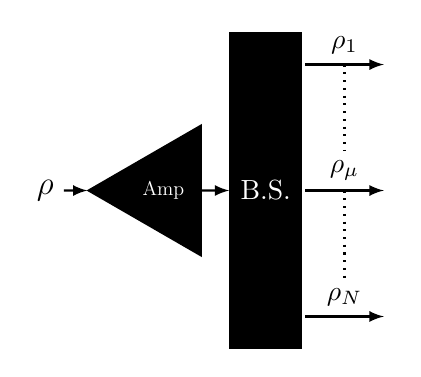
\begin{tikzpicture}[auto, thick, node distance=2.5cm, >=latex]


\node (laptop) {};
% Define the state rho
\node [left of=laptop, node distance=4.3cm] (rho) {\large $\rho$};


% Add BM 
\node [draw, fill=black, minimum width=0.9cm, minimum height=4.cm, right of=rho, node distance=2.8cm] (meas) {\textcolor{white}{B.S.}};

% Add Amp
\node [draw, regular polygon, regular polygon sides=3, shape border rotate=90, fill=black, right of=rho, minimum height=0.3cm, node distance=1.5cm, scale=0.6] (amp) {\large \textcolor{white}{Amp}};


% Connect the nodes
\draw [->] (rho) -- (amp.west);
\draw [->] (amp) -- (meas.west) ;


% Add lines
\draw[->] (-1.,1.6) -- (-0,1.6) node[midway,above] (r1) {$\rho_1$};
\draw[->] (-1.,0) -- (-0,0) node[midway,above] (r2) {$\rho_\mu$};
\draw[->] (-1.,-1.6) -- (-0,-1.6) node[midway,above] (r3) {$\rho_N$};



\draw[-,dotted] (r1.south) -- (r2.north);
\draw[-,dotted] (r2.south) -- (r3.north);


\end{tikzpicture}

\end{document}